\subsection*{導入：ソフトウェア構築とは何か}
\addcontentsline{toc}{subsection}{導入：ソフトウェア構築とは何か}

ソフトウェア構築とは、ソフトウェアを詳細に作成し、保守する活動である。具体的には、コーディング、検証、単体テスト、統合テスト、デバッグを含む。構築は、設計書の内容をただ機械的に写す作業ではない。多くの現場では、詳細な設計判断の一部が構築中に行われる。たとえば、どのデータ構造を使うか、エラーをどこで検出するか、処理をどの関数に分けるか、どのライブラリを使うかは、構築段階で決まることが多い。

この章の知識領域は、他の知識領域と強く結びつく。設計の成果物を入力として使い、テストに渡す成果物を作るため、ソフトウェア設計とソフトウェアテストとの関係が特に強い。また、構築ではソースファイル、テストケース、設定ファイル、文書など多数の構成品目が生まれるため、ソフトウェア構成管理とも密接に関係する。品質、プロジェクト管理、計算基礎とも関係が深い。

\begin{keybox}{重要}
ソフトウェア構築は、実装だけでなく「実装を検証可能にし、変更可能にし、統合可能にし、保守可能にする活動」である。したがって、構築の品質は、完成したソフトウェアの品質だけでなく、後続の変更や運用のしやすさにも影響する。
\end{keybox}

\par\smallskip
\begin{center}
\centering
\IfFileExists{assets/generated_figures/ch04/fig-ch04-02.png}{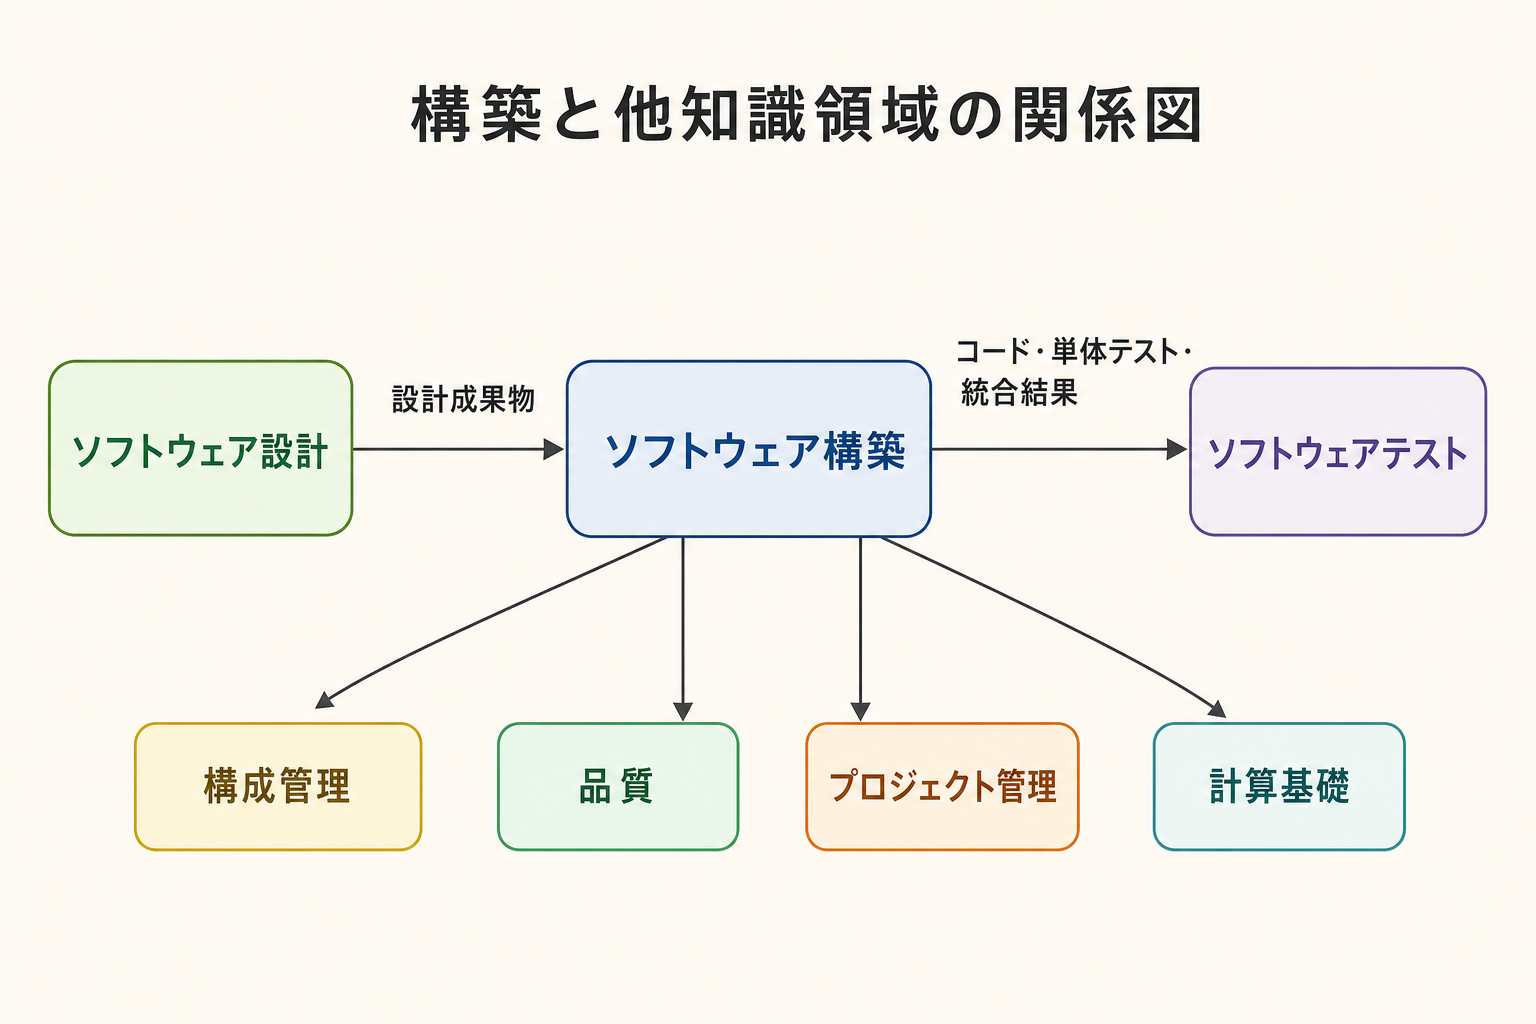
\includegraphics[width=0.96\linewidth]{assets/generated_figures/ch04/fig-ch04-02.png}}{\fbox{\parbox[c][48mm][c]{0.9\linewidth}{\centering 画像生成待ち\\構築と他知識領域の関係図}}}
\par\smallskip
\refstepcounter{figure}\label{fig:ch04-02}図 \thefigure: 構築と他知識領域の関係図
\end{center}
図 \thefigure は、構築と他知識領域の関係図を視覚的に整理したものである。
\par\smallskip
